\section{Dependent Variables}
Participants in this project have been given the freedom to choose their own independent and dependent variables. This resulted in wide variety of variables to be tracked as there were varying interests and varying behavioral changes that participants wanted to experiment on. Below is the list of dependent variables that 21 participants tracked in this project. Please note that some of the variables have been grouped into a particular category. For examples the “Exercise” in the Fig.\ref{fig:variables} includes variables like “Pacing your run”, “Swimming” and “Exercise occurrences”.

\begin{figure}[!t]\centering
%\begin{wrapfigure}{o}{\textwidth}\centering
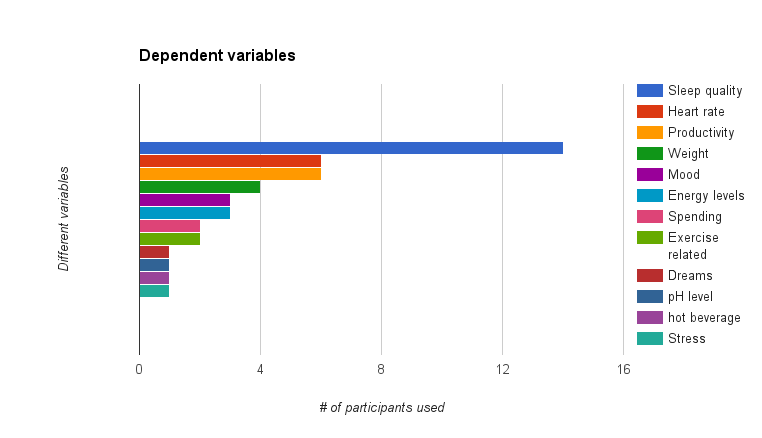
\includegraphics[width=1.0\columnwidth]{images/dependent_variables.png}
\caption{\footnotesize Dependent variables tracked in the class study \label{fig:variables} 
}%\end{wrapfigure}
\end{figure}
%
It is very evident from Fig.\ref{fig:variables} that many participants felt necessary to track their sleep quality. Since the participant group are students of top tier college, it makes sense that sleep is something they care about in their lifestyle amidst loads of deadlines and activities. Also one can note from the previous section that the most of the devices participants used gives sleep quality as their main feature. Hence with sleep quality being the most important factor the participant group cares and it being the most easy variable that can be tracked using the devices, it is no surprise that 14 participants tracked this variable. 

After Sleep quality, Heart rate is another feature that wearable devices care to track about. With increasing heart diseases globally, this is one of most used metric to show if a person is healthy. Hence Heart rate is a variable that participants had easy access to and wanted to know the changes it had on their behavioral changes.

Productivity is a variable that participant group cared about as it is something that they want to improve on a daily basis in one form or the other. Factors that determine productivity varies from individual to individual and tracking devices fail to capture this personalized subjective variable. Hence participants came up with interesting self reporting techniques that will be discussed in detail in section.

Weight is another variable that participant group cared to track with respect to their behavior changes. Weight has been traditionally something that people cared in terms of that affecting their appearance and also it being a good metric to judge your health status. So it came out to be one of the obvious variables that participant group chose in this experiment. 

Though there are other interesting variables people tracked during the experiment. this paper will focus on the top 4 variables and discuss insights and observations from the participants in detail.

\begin{figure*}[!t]\centering
%\begin{wrapfigure}{o}{\textwidth}\centering
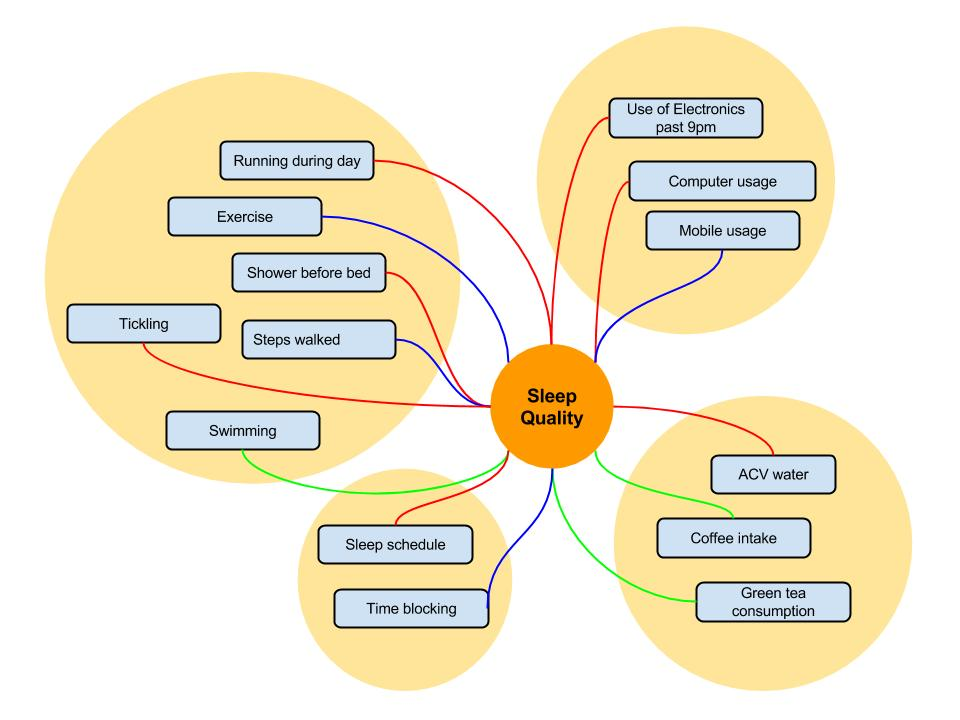
\includegraphics[width=0.47\textwidth]{images/Sleep_quality.jpg}
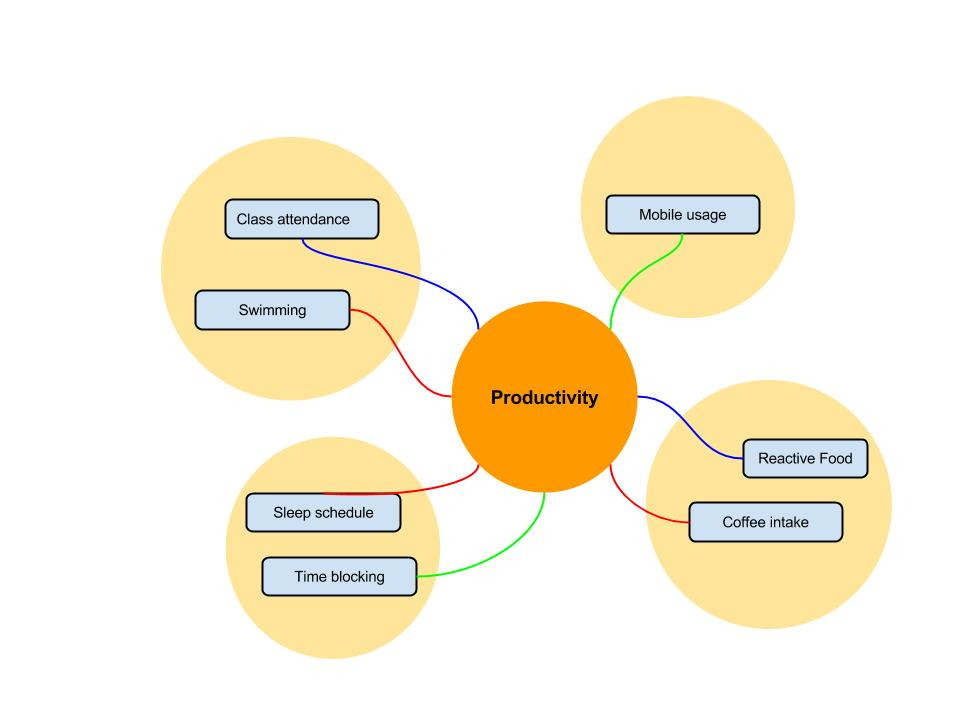
\includegraphics[width=0.47\textwidth]{images/Productivity.jpg}
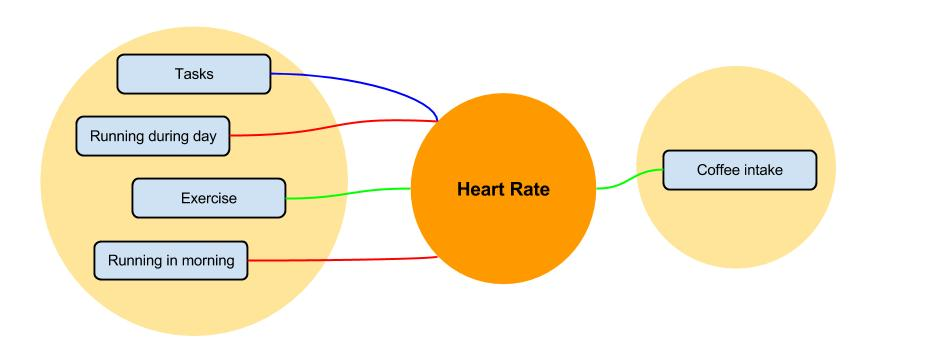
\includegraphics[width=0.47\textwidth]{images/Heart_rate.jpg}
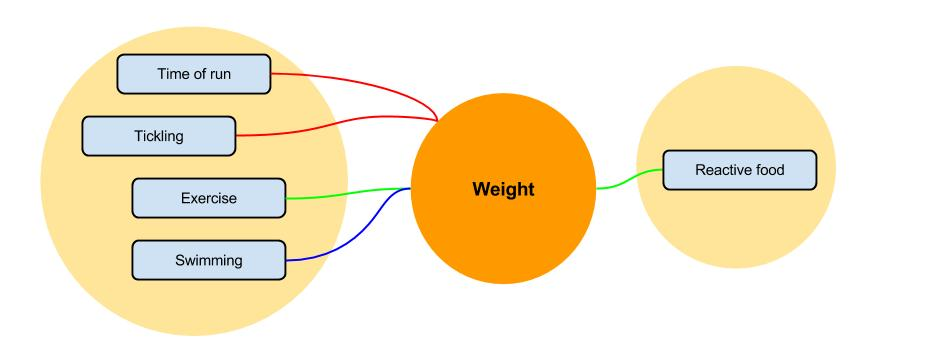
\includegraphics[width=0.47\textwidth]{images/Weight.jpg}
\caption{\footnotesize Dependent variables and the independent variables that were related to it by the participants \label{fig:dependentvsindependent} 
}%\end{wrapfigure}
\end{figure*}

\subsection{Sleep quality}
For tracking sleep, participants used various applications and devices from Sleep As Android to FitBit which kept track of the amount of time people were in various levels of sleep (light, deep, R.E.M.) and how many times they woke up during the night. Devices have various approaches to measuring sleep quality. Mobile apps use ambient noise and movements in the bed to measure the sleep quality. Some wearable devices use body movements and others use a pulse sensor to measure sleep quality. The quality of the measurements is directly proportional to the cost of the device and hence the reported sleep quality measurements are approximations. 

It is interesting to see what each participant’s hypothesis were and the independent variables that they hypothesized to affect sleep quality. Below figure shows all the independent variables that were reported directly related to sleep quality by the participants. The independent variables have been clustered into categories “usage of devices”, “activities”, “schedule changes” and “consumption of drinks”. The green edges indicates that these variables affect sleep quality. The red edge indicates that these variables do not have an effect on the sleep quality. The blue edge indicates that the experiments on these variables have not had any conclusion due to less data points.

For the most part, least number (3) of variables seem to have affected sleep. Most of all the hypotheses (7) have been rejected by the participants. Significant number of hypotheses were inconclusive (4). 

A common observation from the reports of the participants is that their hypothetical behavior that affects the sleep quality is not always true. For example, activities (except swimming) and device usage had no effect on the sleep quality as observed by the participants. Also one would certainly assume that a better schedule of the day will improve the sleep quality, but its been proven otherwise in this study. These are some interesting insights about the factors affecting sleep quality. 

But one must note that, all these are conclusions highly biased to the individuals and their tracking methods. If every participant used a single common tracking mechanism to track the sleep quality, then it is easy to conclude in general that a particular behavior either improves or worsens the sleep quality. However with constraint on the number of days and experimental design one can adopt, some of these conclusions have given insights of what variables one might want to consider when they are tracking their sleep quality.

Some interesting observations by the participants are: a) one participant had trouble falling asleep once they restricted their use of electronics, so they started reading to fill the time; b) one participant woke up more according to their findings; c) one of the user had seen improvement of 29% in the sleep quality when they swam in the night between 9-10:30pm. 

Others did not come to a conclusion because they felt the the variable was not properly tracked, for example, mobile devices were not as reliable in tracking sleep in comparison to wearable device. Some of the wearable devices track the motion of the hand to measure the sleep time and that could also be noisy and not accurate. So it may be the case that the data points has to be definitely more than 28 days to come to any conclusion on this regard. In addition to this the users are supposed to design their experiment in AB, ABA, ABAC etc format so they have less data points to the significant change they are tracking and I feel that the “Jet-lag” pointed by one of the participant plays a significant role in producing the transition data.

\subsection{Productivity}


Productivity is a subjective variable and in order to quantify, participants used metrics created based on the completeness of anticipated tasks, “productivity pulse” through RescueTime software, 1-10 scale based on time, 1-7 based on concentration intensity. Some of the apps and plugins used were RescueTime Plugin  and TimeStats Plugin.

Below is the graph show how the independent that variables were related to the Productivity and its outcome at the end of the experiment.

As shown above, except for “Mobile usage” and “Time blocking,” all the other independent variables either didn’t have any impact on the productivity or their data points were not enough to conclude any claims.

As far as tracking productivity went, this was one of the most subjective processes.  There is no set metric for productivity nor were there any concrete ways in tracking it.  Across the different studies, productivity was in most cases a self reported process of doing work, through which each student employed some metric to express daily productivity.  This seems acceptable, as every person works differently, encounters personal setbacks and ranges in their times of productivity (whether it's failing to complete a task or taking too long on a task or getting distracted) and presumably, their chosen methods of data collection and analysis were the ones that fit their perceptions of productivity best.  A common issue encountered with the trackers of productivity was spring break.  Unlike with an action or measurable effects (such as heart rate or weight), productivity is very dependent upon the status of the experimenter’s life.  As spring break arrived, the nature of the work needed to be done changes along with students’ schedules, rendering parts of time either harder to analyze or irrelevant to the study.  There were mixed results in the effects of different variables’ effects on productivity.  One user found the method of time blocking to be instrumental in significantly increasing their productivity (20-40), while independent variables such as swimming or a fixed sleep schedule did not produce statistically significant changes in productivity.  Class attendance had a significant correlation with productivity and data was just shy of being able to statistically prove it increased the experimenter’s productivity. 

Most importantly defining what is productive is first step in this experiment as experienced by the participants. It needs to be decided what counts as being productive for themselves. Is doing homework productive? Is cooking lunch or checking and answering emails productive? There are various layers and it’s difficult to understand what really is productive to you. Perhaps going to bed instead of staring at that math problem for three hours is more productive. After deciding what constitutes as productive to the user, perhaps they must also decide how intense the work is and how that might affect your data as one user pointed out. Overall, productivity is difficult to keep track of because it’s difficult to quantify an hour of doing mindless work to thirty minutes of intense focused problem solving. 

One common tracking mechanism people had was to self report their activities. Some tools that has helped are reminders from apps like Reporter with some questionnaires about what they did the previous hour? How would they rate their productivity? and so on. Hence there may be significant roles these apps can play to track the productivity. Also tools on desktop to track the amount of time you were on a particular website can in turn give you the details of how many hours have you spent distracted. This also helps the user at the end of the day know how much time he has spend not working on the activity he has to focus on. So there are many tools that can track various aspects of productivity and in consensus with each other based on the logged data can precisely tell the productivity in a day. This is something one could focus to improve upon in Personal informatics domain.

\subsection{Heart rate}
Heart rate is measured either using a wearable tracking device that has special sensors or physically by recording the pulse of a hand. Participants used both these methods in their tracking experiment. 
Below is the graph show how the independent variables were related to the Heart rate and its outcome at the end of the experiment.

Exercise and Coffee intake has an impact on the heart rate. One of the participant made an interesting observation that Coffee intake increases the heart rate immediately after the consumption. Activities overall doesn’t improve the heart rate. Running in different time of the day doesn’t have any impact on the overall heart rate in a day. Participants are in age group of early and mid 20s and so there was no abnormal observations that were made. 

\subsection{Weight}

This being a physical measurement, everyone used the standard scale. Below is the graph show how the independent variables were related to the Weight and its outcome at the end of the experiment.
It can be noticed from above graph that except “Exercise” and “Reactive food” non other independent variables had an impact on weight. “Swimming” didn’t have significant effect on the weight and hence it was declared inconclusive. Overall weight as everyone knows is directly dependent on the food intake and the exercise. Weight is one of the most common factors that people would like to consider since being too fat contributes to hypertension, diabetes and some other diseases while being too skinny may cause to lose self-confidence. 

Some important observations are: a) One of the user showed that there is weight gain once he switched to post-6PM runs; b) One user noticed that the weight measured in the morning is significantly lower compared to the weight of the body in the night. But none of the experiments have been super conclusive. Tracking the weight is not a noisy/uncertain like other variables we discussed in this section, but an increased duration of the study might have given more conclusive insights.

